\textbf{1. Assumptions.} I use a uniform, linearly elastic Euler--Bernoulli beam with small transverse displacement and slope. Cross sections remain plane and normal to the neutral axis. Shear deformation and rotary inertia are neglected, and the reference axis passes through the centroid. The notation and sign convention follow the course notes, PDF pages 172--176.

\textbf{2. Free-body diagram.} The element free-body diagram below follows the sign convention of the notes. Its left face carries $N$, $M$, and $V$, while the right face carries $N+N_x\,dx$, $M+M_x\,dx$, and $V+V_x\,dx$. Opposite directions on the two faces yield the signed resultants below.
\begin{figure}[H]
\centering
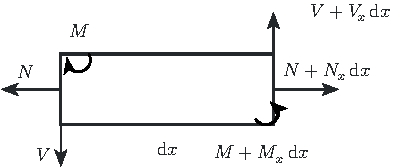
\includegraphics[width=0.65\linewidth]{figures/generated/solutions/B1-fbd.pdf}
\caption{Stress resultants on an infinitesimal beam element.}
\end{figure}

\textbf{3--5. Stress resultants and kinematics.} For longitudinal stress $\sigma=E\epsilon$ and area $A$,
\[
N=\int_A\sigma\,dA=E\int_A\epsilon\,dA,\qquad
M=-\int_A z\sigma\,dA=-E\int_A z\epsilon\,dA.
\]
Plane sections give $u=-zw_x$ and $\epsilon=u_x=-zw_{xx}$. Since $\int_Az\,dA=0$ and $I=\int_Az^2\,dA$,
\[
\boxed{N=0,\qquad M=EIw_{xx}.}
\]

\textbf{6--10. Element balance.} Using the directions in the supplied free-body diagram and retaining first-order terms in $dx$,
\[
\sum F_z=V_x\,dx,\qquad
\sum M=(M_x+V)\,dx.
\]
Newton's law gives $V_x=mw_{tt}$, while neglected rotary inertia gives $M_x+V=0$. Thus $V=-M_x=-EIw_{xxx}$ and
\[
\boxed{EIw_{xxxx}+mw_{tt}=0.}
\]

\textbf{11--15. Harmonic motion.} The course notes define the flexural constant and wavenumber by
\[
a=\left(\frac{EI}{m}\right)^{1/4},\qquad
a^4w_{xxxx}+w_{tt}=0,\qquad
\gamma=\frac{\sqrt{\omega}}{a}.
\]
Substituting $w=W(x)e^{-i\omega t}$ gives
\[
a^4W''''-\omega^2W=0,\qquad W''''-\gamma^4W=0.
\]

\textbf{16--21. Characteristic roots and general solution.} Substitution of $W=e^{sx}$ gives $s^4-\gamma^4=0$, with $s=\pm i\gamma,\pm\gamma$. Therefore
\[
W=A_1e^{i\gamma x}+A_2e^{-i\gamma x}+A_3e^{\gamma x}+A_4e^{-\gamma x}
\]
or, with a new set of constants,
\[
\boxed{W=C_1\sin\gamma x+C_2\cos\gamma x+C_3\sinh\gamma x+C_4\cosh\gamma x.}
\]
Four boundary conditions determine the constant ratios and allowed frequencies for free vibration. A nonzero mode has arbitrary scale, which is fixed by normalization or initial conditions. Forced vibration uses the boundary conditions and the forcing to determine the absolute coefficients.
